Convolutional neural networks were first proposed for the image recognition by Y.LeCun \cite{lecun1989backpropagation}, 
but gained recognition after the 
ImageNet 2012 competition \cite{krizhevsky2012imagenet}. 
In this work we use 3D convolutional networks to score protein structures. The network consists of 
basic layers that transform the input.
The schematic representation of the model architecture is shown on the Fig \ref{Fig:CNNModel}.
It is comprised of three blocks of alternating convolutional, 
volumetric batch normalization and ReLU layers and three 
fully connected layers with ReLU nonlinearities. The final output of the network is a single number, 
that is interpreted as a score of an input structure. Further we provide a consize description of each layer.

\begin{figure}[H]
    \centering
    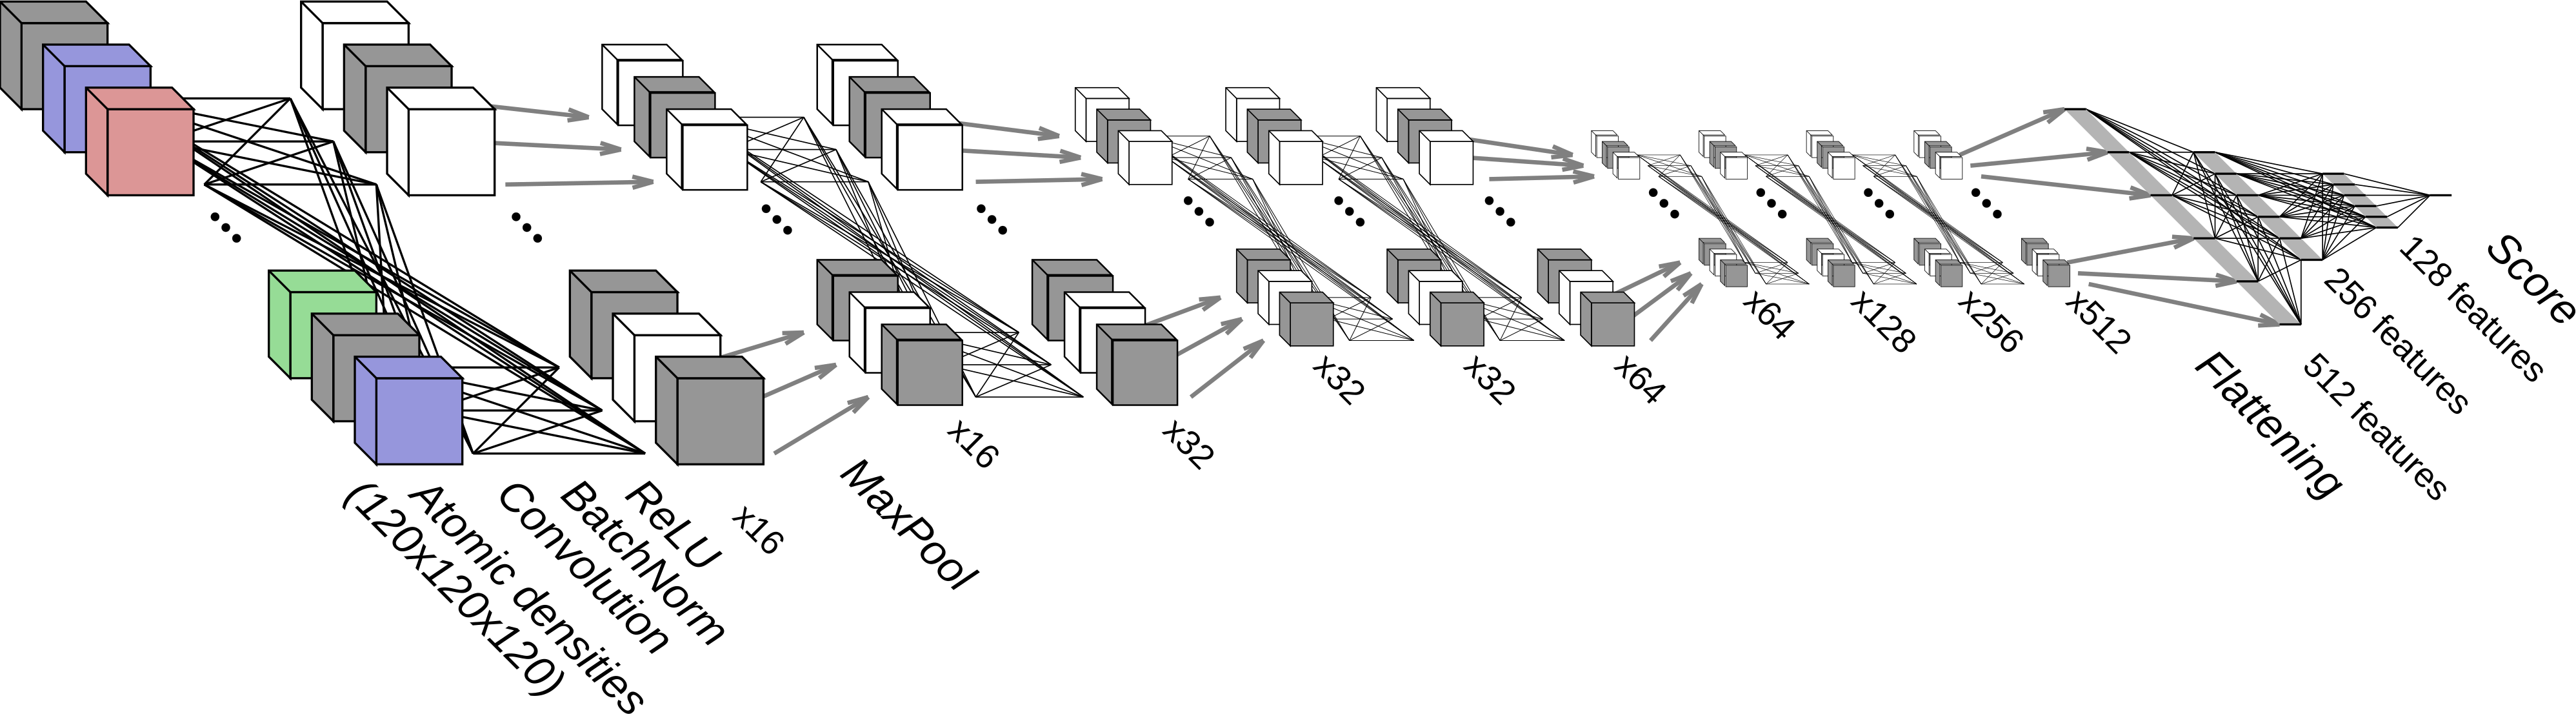
\includegraphics[width=\linewidth]{Fig/ConvnetDiagramV1.png}
    \caption{The schematic representation of the convolutional neural network architecture used in this work. 
    The arrows between the boxes denote maximum pooling layers and the connections denote 
    consequent 3d convolutional, batch normalization and ReLU layers. The numbers xM denote the number of filters 
    used in the corresponding 3d convolutional layer. The size of all filters and 
    maximum pooling domains are 3x3x3. The grey stripes denote one-dimensional vectors and crossed lines between them 
    stand for fully-connected layer with ReLU non-linearities. The details of the model parameters can be found in 
    Supplementary Information.}
    \label{Fig:CNNModel}
\end{figure}

The 3D convolutional layer takes $N$ input density maps and transforms them using $M$ filters
according to the following formula:
$$
f^{out}_i (\mathbf{r}) = \sum^{N}_{j=1} \int F_i (\mathbf{r} - \mathbf{\tau}) \cdot f^{in}_j(\mathbf{\tau}) ~d\tau, i \in [1,M]
$$
where filters are denoted using $F_j$. In standard implementations convolutions are approximated by the sum on a grid.
The ReLU nonlinearity is computed in the following way:
$$
f^{out}_i (\mathbf{r}) = \begin{cases}
               f^{in}_i(\mathbf{r})& f^{in}_i(\mathbf{r})\geq 0\\
               0                 &f^{in}_i(\mathbf{r})<0\\
            \end{cases}, i \in [1,M]
$$
The batch normalization layer was introduced by S.Ioffe and C.Szegedy \cite{ioffe2015batch} to address the problem of internal convariate shift:
the change in the distribution of subnetwork outputs due to the change in its parameters during the training. In practice, this layer takes the 
input and normalizes its values according to the mean values and variances of the corresponding values in the subset of examples used to estimate 
the gradient (minibatch):
$$
    \hat{f}^{in}_i(\mathbf{r}) = \frac{f^{in}(\mathbf{r}) - \mu_{B}}{\sqrt{\sigma^{2}_{B} + \epsilon}}, i \in [1,N_B]
$$
where $\mu_B(\mathbf{r}) = \frac{1}{N_B} \sum_{i=1}^{N_B} f^{in}_i(\mathbf{r})$ and 
$\sigma^{2}_{B} = \frac{1}{N_B} \sum_{i=1}^{N_B} \left( f^{in}_i(\mathbf{r}) - \mu_B (\mathbf{r}) \right)$. 
The constant $\epsilon$ is added to avoid division by zero, the number of 
examples in the minibatch is denoted as $N_B$. Afterwards, the output of this layer is computed by scaling the normalized inputs:
$$
f^{out}_i(\mathbf{r}) = \gamma \hat{f}^{in}_i(\mathbf{r}) + \beta, i \in [1,N_B]
$$
The parameters $\gamma$ and $\beta$ are learned along with other parameters of the network during the training.

The maximum pooling layer (MaxPool) is used to build a coarse-grained representation of the input. The output of this layer is 
the maximum over the cubes of the size $d$, that cover the input domain without overlapping. 
The output data domain is then $d$ times smaller than the input data box.

During the coarse-graining procedures the size of the input data box eventually shrinks to a single cell. The flattening layer reshapes the array of 
3d density maps to a single vector.

Afterwards, we compute several transformations using fully-connected layers. These layers transform a vector $\mathbf{x_{in}}$ in the follosing way:
$$
x_{out} = \mathbf{W} \cdot x + \mathbf{b}
$$
where $\mathbf{W}$ is a matrix and $\mathbf{b}$ is a vector, that are learned during the training.
